% Provenance (never printed): old terminale S material on the disappearance of
% mountain ranges (erosion, transport, sedimentation, isostatic rebound, the
% recycling of continental material). Owner (Sync 0/1): denudation rate,
% sediment load (bed, suspended, dissolved), isostatic rebound, detrital rock,
% diagenesis. Weathering, erosion, deposition are Book 1's (g5); hydrolysis and
% clay minerals g10.07's; discharge g10.08's; isostasy and Airy's model g11.03's;
% sedimentary basin g11.09's; mountain root g12.01's; metamorphism g12.03's;
% half-life is physics' (recalled in prose). Figures: figdata/grade-12/relief_decay.py
% (rates, decay curves, the Varden unconformity from figdata/shared/region.py).
\chapter{Hancurnya Pegunungan}\label{ch:g12:destruction-of-mountains}

Dilihat dari Stasiun Antariksa Internasional, Pegunungan Appalachia di
Amerika Utara bagian timur membentuk pola yang mencolok: punggung-punggung
bukit yang panjang, gelap, dan berhutan, berselang-seling dengan lembah-lembah
pertanian yang pucat, lebih dari \qty{500}{km} panjangnya pada foto di bawah.
Punggung-punggung itu adalah lapisan batuan keras yang terlipat rapat ketika
Afrika mendorong Amerika Utara, pada zaman Karbon dan Perm, lebih dari 250 juta
tahun yang lalu. Kini puncak tertingginya, Gunung Mitchell, titik tertinggi di
timur Sungai Mississippi, menjulang \qty{2037}{m} di atas permukaan laut,
kurang dari seperempat tinggi Everest.
% ledger: photo:g12-appalachians, usgs:alleghanian, usgs:alleghanian-age, ics:base.Triassic, ncparks:mitchell (6684 ft), tht:everest (Book 1 row, 8848.86 m)

\begin{omfigure}
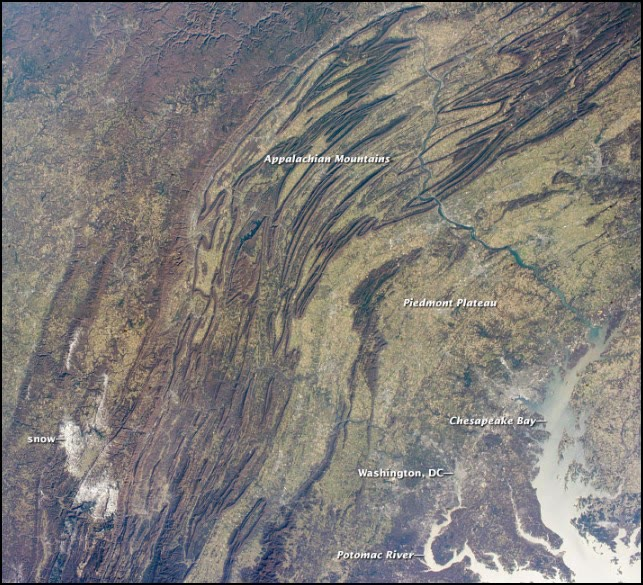
\includegraphics[width=0.6\linewidth]{images/book2/g12-iss-appalachians.jpg}

{\small Pegunungan Appalachia bertipe lembah-dan-punggungan, dari Pennsylvania
timur laut (kanan atas) sampai Virginia Barat, dipotret dari Stasiun Antariksa
Internasional pada 17 November 2012. Punggung-punggung berhutan itu adalah
lapisan batuan keras, lembah-lembah pertaniannya lapisan yang lebih lunak. Foto
NASA (domain publik).}
\end{omfigure}
% ledger: photo:g12-appalachians

Sebuah pegunungan tidak bertahan selamanya. Sejak saat ia naik, hujan, es, dan
sungai menyerangnya; batuan yang mereka angkut akhirnya sampai di laut, tempat
batuan itu menjadi batuan baru. Bab ini mengukur seberapa cepat hal itu
terjadi, mengikuti puing-puingnya sampai ke tempat ia berubah menjadi batu, dan
menunjukkan mengapa pegunungan yang sedang terkikis terus naik selama proses
itu.

\begin{recall}
Pelapukan menghancurkan batuan di tempatnya; erosi mengangkut puing-puingnya,
dan pengendapan meletakkannya di tempat lain (Buku 1, kelas 5). \omterm{def:g10:soil-formation:chemical-weathering}{Pelapukan kimia}
mengubah feldspar menjadi \omterm{def:g10:soil-formation:clay}{mineral lempung} melalui \omterm{def:g10:soil-formation:hydrolysis}{hidrolisis}
(\cref{ch:g10:soil-formation}). \omterm{def:g10:drainage-basins:discharge}{Debit} sebuah sungai adalah volume air yang
melewati suatu titik dalam satu detik (\cref{ch:g10:drainage-basins}). Kerak
mengapung di atas mantel dalam \omterm{def:g11:lithosphere-asthenosphere:isostasy}{isostasi}; dalam model Airy, wilayah yang
keraknya lebih tebal $\Delta H$ berdiri lebih tinggi
$\Delta H\,(\rho_m - \rho_c)/\rho_m$
(\cref{ch:g11:lithosphere-asthenosphere}), dan pegunungan yang tinggi bertumpu
pada akar dari kerak yang tebal (\cref{ch:g12:continental-crust}). Sedimen
menumpuk di dalam \omterm{def:g11:fossil-fuel-geology:basin}{cekungan sedimen} (\cref{ch:g11:fossil-fuel-geology}). Batuan
yang terkubur dalam di sebuah sabuk pegunungan termetamorfosis
(\cref{ch:g12:metamorphic-rocks}).
\end{recall}

\section{Seberapa cepat daratan terkikis?}

\begin{definition}[Laju denudasi]\label{def:g12:destruction-of-mountains:denudation}
Yang disebut \emph{laju denudasi}\index{laju denudasi} sebuah wilayah adalah
tebal rata-rata batuan yang dihilangkan dari wilayah itu oleh pelapukan dan
erosi bersama-sama per satuan waktu. Laju itu biasanya dinyatakan dalam meter
per sejuta tahun (\unit{m/Ma}), sama dengan milimeter per seribu tahun.
\end{definition}
% ledger: pb11:rates (rates in m/Myr), earle:loads

Bagaimana mengukur sesuatu yang begitu lambat? Sinar kosmik yang menghantam
tanah membentuk sebuah isotop langka, berilium-10, di dalam kuarsa beberapa
meter teratas batuan. Makin lambat sebuah permukaan terkikis, makin lama
setiap butir tinggal di dekat permukaan, dan makin banyak berilium-10 yang
dikumpulkannya. Mengukurnya di dalam pasir sebuah sungai memberikan \omterm{def:g12:destruction-of-mountains:denudation}{laju
denudasi} rata-rata seluruh cekungan di hulunya, selama ribuan sampai jutaan
tahun terakhir.
% ledger: pb11:rates (10Be produced within a few metres of the surface; concentration reflects near-surface residence time; 10^3 to 10^6 years)

Sebuah kompilasi atas 1599 pengukuran seperti itu mendapati bahwa singkapan
batuan yang telanjang terkikis lambat, rata-rata \qty{12}{m/Ma} (median
\qty{5.4}{m/Ma}), dan tidak pernah lebih cepat dari \qty{140}{m/Ma}. Seluruh
\omterm{def:g10:drainage-basins:drainage-basin}{daerah aliran sungai} kehilangan jauh lebih banyak, rata-rata \qty{218}{m/Ma},
tetapi dengan median hanya \qty{54}{m/Ma}: beberapa cekungan yang cepat
menarik rata-ratanya ke atas. Yang tercepat adalah yang curam: kemiringan
rata-rata sebuah cekungan adalah faktor yang paling baik meramalkan lajunya.
Cekungan di wilayah yang aktif secara seismik, tempat pegunungan sedang naik,
terkikis sekitar dua kali lebih cepat daripada cekungan di wilayah yang tenang.
% ledger: pb11:rates

\begin{omfigure}
\begin{tikzpicture}
\begin{axis}[omrecord, xbar, xmode=log, log origin=infty, bar width=7pt, bar shift=0pt,
  width=0.62\linewidth, height=6.6cm, scale only axis, xmin=3, xmax=1000,
  ymin=0.4, ymax=10.6, ytick={1,...,10}, y tick label style={font=\scriptsize, align=right},
  yticklabels={{singkapan, median}, {singkapan, rata-rata}, {sungai dunia (neraca)}, {cekungan, median},
    {Mississippi, sebelum 1900 (neraca)}, {cekungan kering, rata-rata}, {cekungan tenang, rata-rata}, {cekungan, rata-rata},
    {cekungan aktif seismik, rata-rata}, {cekungan kutub, rata-rata}},
  xlabel={laju denudasi (\unit{m/Ma}), skala logaritmik}, ymajorgrids=false,
  unbounded coords=discard, nodes near coords, nodes near coords align={horizontal}, nodes near coords style={font=\scriptsize},
  point meta=rawx, every node near coord/.append style={/pgf/number format/.cd, fixed, precision=0}]
% computed in figdata/grade-12/relief_decay.py; ledger: pb11:rates, mm10:mississippi, kammerer:mississippi, earle:loads, cm95:crust
\addplot[fill=omThm!45, draw=omThm, every node near coord/.append style={/pgf/number format/.cd, fixed, precision=1}] table[x=measured, y=idx] {figdata/out/grade-12-relief_decay-rates.dat};
\addplot[fill=omDef!45, draw=omDef] table[x=budget, y=idx] {figdata/out/grade-12-relief_decay-rates.dat};
\end{axis}
\end{tikzpicture}

{\small \omterm{def:g12:destruction-of-mountains:denudation}{Laju denudasi} yang diukur dengan berilium-10 (merah: 1599 pengukuran,
1149 di antaranya di dalam pasir sungai) dan dua laju yang dihitung dalam bab
ini dari sedimen yang diangkut sungai (biru). Sumber: Portenga dan Bierman
(2011); Meade dan Moody (2010); Syvitski dan kawan-kawan (2005).}
\end{omfigure}
% values: world_m_per_myr 43.5, miss_before_1900_m_per_myr 55.8 (relief_decay.py)

\section{Sungai mengangkut pegunungan pergi}

Sebagian besar yang terkikis dari daratan meninggalkannya lewat sungai.

\begin{definition}[Muatan sedimen]\label{def:g12:destruction-of-mountains:load}
Yang disebut \emph{muatan sedimen}\index{muatan sedimen} sebuah sungai adalah
bahan yang diangkutnya, dalam tiga bentuk: \emph{muatan dasar}\index{muatan dasar},
butir-butir besar yang digulirkan, didorong, atau dilompatkan di
sepanjang dasar; \emph{muatan suspensi}\index{muatan suspensi}, butir-butir
kecil yang tertahan di dalam air yang bergerak; dan \emph{muatan
terlarut}\index{muatan terlarut}, ion-ion dalam larutan, seperti kalsium dan
klorida, yang ditinggalkan oleh \omterm{def:g10:soil-formation:chemical-weathering}{pelapukan kimia}.
\end{definition}
% ledger: earle:loads

Rata-rata, \omterm{def:g12:destruction-of-mountains:load}{muatan terlarut} sekitar \qty{15}{\percent} dari massa yang diangkut
sebuah sungai. Makin cepat airnya, makin besar butir yang dapat diangkatnya.
Sebutir pasir berdiameter \qty{1}{mm} terangkat dari dasar pada sekitar
\qty{20}{cm/s}, dan begitu bergerak ia tetap melayang sampai arus melambat di
bawah \qty{10}{cm/s}. Butir lanau lebih sulit diangkat daripada pasir, karena
saling melekat: butir berukuran \qty{0.01}{mm} memerlukan \qty{60}{cm/s} untuk
terangkat, tetapi sesudah itu arus \qty{0.1}{cm/s} sudah cukup untuk
membuatnya tetap melayang. Itulah sebabnya sungai yang banjir berwarna cokelat,
dan lumpur yang paling halus menempuh perjalanan sampai ke laut.
% ledger: earle:loads

\begin{omfigure}
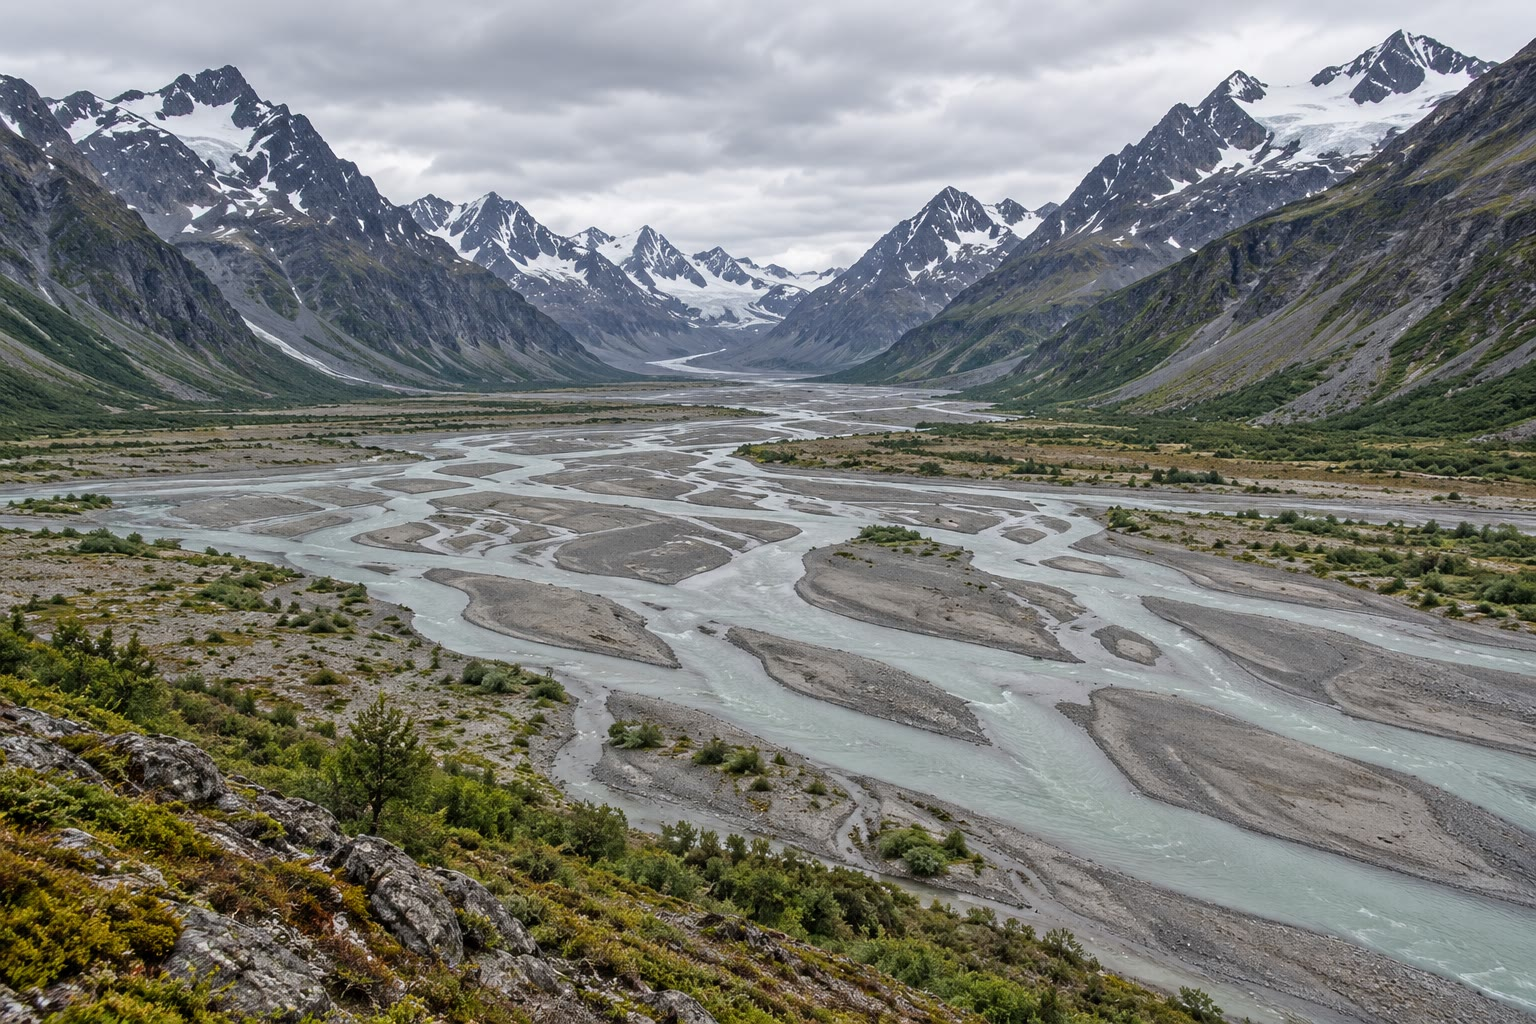
\includegraphics[width=0.66\linewidth]{images/book2/ai/g12-braided-river.jpg}

{\small Sungai teranyam di sebuah lembah pegunungan glasial: alur-alur dangkal
memisah dan bergabung kembali di antara gosong-gosong kerikil yang hanya
dipindahkan air ketika banjir. (ilustrasi AI)}
\end{omfigure}

Mengukur apa yang diangkut sebuah sungai memberikan cara kedua untuk mencari \omterm{def:g12:destruction-of-mountains:denudation}{laju denudasi}.

\begin{method}[Neraca erosi]\label{met:g12:destruction-of-mountains:budget}
\begin{enumerate}
  \item Ambillah massa sedimen yang diangkut sungai dalam setahun, lalu
        tambahkan \omterm{def:g12:destruction-of-mountains:load}{muatan terlarutnya} (bila hanya muatan padatnya yang
        diketahui, bagilah dengan $0.85$).
  \item Bagilah dengan massa jenis batuan, sekitar \qty{2830}{kg/m^3} untuk
        \omterm{def:g12:continental-crust:continental-crust}{kerak benua}, untuk mendapatkan volume batuan yang dihilangkan setiap
        tahun.
  \item Bagilah dengan luas \omterm{def:g10:drainage-basins:drainage-basin}{daerah aliran sungai}: hasilnya adalah tebal yang
        dihilangkan setiap tahun.
  \item Kalikan dengan $10^6$ untuk menyatakannya dalam meter per sejuta tahun.
\end{enumerate}
\end{method}
% ledger: earle:loads, cm95:crust

\begin{example}[Sungai Mississippi]\label{ex:g12:destruction-of-mountains:mississippi}
Sebelum 1900, sistem sungai Missouri--Mississippi mengangkut sekitar 400 juta
ton sedimen setahun ke laut, dari cekungan seluas sekitar
\qty{2980000}{km^2}. Dengan \omterm{def:g12:destruction-of-mountains:load}{muatan terlarutnya}, $400/0.85 \approx 471$ juta
ton, yaitu $\num{4.71e11}/2830 \approx \qty{1.66e8}{m^3}$ batuan setahun.
Bila disebarkan di atas $\qty{2.98e12}{m^2}$, itu adalah selapis
\[
  \frac{\num{1.66e8}}{\num{2.98e12}} \approx \qty{5.6e-5}{m}
  \text{ setahun, sekitar } \qty{56}{m/Ma}.
\]
Antara 1987 dan 2006 sungai itu hanya mengangkut 145 juta ton setahun, yang
memberikan sekitar \qty{20}{m/Ma}: bendungan-bendungan yang dibangun di Sungai
Missouri pada tahun 1950-an menahan sekitar 100 sampai 150 juta ton setahun,
dan bangunan-bangunan lain menahan lebih banyak lagi.
\end{example}
% ledger: mm10:mississippi, kammerer:mississippi, earle:loads, cm95:crust
% values: miss_before_1900_m_per_myr 55.8, miss_1987_2006_m_per_myr 20.2 (relief_decay.py)

Neraca yang sama dapat dibuat untuk seluruh dunia. Sebelum manusia mengubah
sungai-sungai, sungai mengangkut sekitar 15.5 miliar ton sedimen padat setahun
ke pantai; dengan \omterm{def:g12:destruction-of-mountains:load}{muatan terlarutnya}, itu sekitar \qty{6.4}{km^3} batuan
setahun, yang diambil dari \qty{1.48e8}{km^2} benua: \omterm{def:g12:destruction-of-mountains:denudation}{laju denudasi} rata-rata
sekitar \qty{43}{m/Ma}, dekat dengan median pengukuran berilium-10. Sejak itu
manusia telah mengubah kedua sukunya: erosi tanah telah menambah apa yang
diangkat sungai sekitar 2.3 miliar ton setahun, tetapi lebih dari 100 miliar ton
sedimen kini tertahan di belakang bendungan.
% ledger: syvitski:modern-flux (Book 1 row, prehuman 15.5 Gt/yr with bed load), sy05:humans, data:etopo1 (land fraction 0.290, grade-11 hypsometry), cm95:crust
% values: world_volume_km3_per_yr 6.44, land_area_km2 1.48e8, world_m_per_myr 43.5 (relief_decay.py)

\section{Dari sedimen menjadi batuan}

Apa yang diangkut sungai diendapkan di tempat arus melambat: di lembah dan
danau, di delta, dan terutama di cekungan-cekungan sedimen di tepi benua.
Lapis demi lapis, sedimen itu terkubur, dan perlahan-lahan berubah menjadi
batuan.

\begin{definition}[Batuan detritus; diagenesis]\label{def:g12:destruction-of-mountains:diagenesis}
Yang disebut \emph{batuan detritus}\index{batuan detritus} (atau batuan
klastik) adalah batuan sedimen yang tersusun dari pecahan-pecahan, yaitu klas,
batuan dan mineral yang lebih tua. Yang disebut
\emph{diagenesis}\index{diagenesis} adalah rangkaian perubahan yang mengubah
sedimen yang terkubur menjadi batuan pada suhu rendah: \emph{kompaksi}, ketika
berat lapisan di atasnya memeras keluar air dan udara, lalu \emph{sementasi},
ketika mineral-mineral yang mengkristal dari air di dalam pori (kalsit, kuarsa,
hematit, \omterm{def:g10:soil-formation:clay}{mineral lempung}) merekatkan butir-butirnya.
\end{definition}
% ledger: earle:clastic

\omterm{def:g12:destruction-of-mountains:diagenesis}{Batuan detritus} dinamai menurut ukuran klasnya:
\begin{itemize}
  \item \textbf{konglomerat} tersusun dari klas membulat yang lebih besar dari
        \qty{2}{mm}, \textbf{breksi} dari klas yang menyudut;
  \item \textbf{batu pasir} tersusun dari pasir, butir antara \qty{2}{mm}
        dan \qty{0.063}{mm}, paling sering berupa kuarsa, mineral yang paling
        tahan terhadap pelapukan;
  \item \textbf{batu lumpur} mengandung setidaknya \qty{75}{\percent} lanau
        dan lempung; batuan itu disebut serpih bila terbelah menjadi
        lapisan-lapisan tipis.
\end{itemize}
% ledger: earle:clastic

\begin{omfigure}
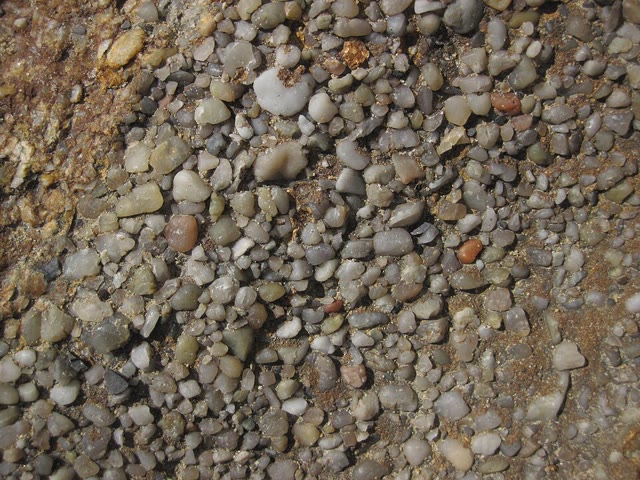
\includegraphics[width=0.5\linewidth]{images/book2/g12-stjohn-conglomerate.jpg}

{\small Konglomerat kerikil kuarsa dari Ohio, berumur Karbon: kerikil kuarsa
yang membulat, disemen oleh pasir yang lebih halus. Foto James
St.~John (CC~BY~2.0).}
\end{omfigure}
% ledger: photo:g12-conglomerate, ics:base.Carboniferous, ics:base.Permian (Lower Pennsylvanian lies in the Carboniferous)

Klas-klas itu merekam perjalanannya. Kerikil yang membulat telah menggelinding
jauh di dalam sungai atau di pantai; kerikil yang menyudut nyaris tidak
berpindah. Batu pasir yang hampir seluruhnya terdiri dari kuarsa berasal dari
batuan yang lama terlapuk, sampai mineral-mineral lainnya telah menjadi lempung.
% ledger: earle:clastic (rounded/angular, most sand grains quartz, the most resistant mineral)

\section{Akarnya naik}

Bila erosi hanya menghilangkan batuan dari puncak sebuah pegunungan, pegunungan
setinggi \qty{2}{km} yang terkikis dengan laju \qty{200}{m/Ma} akan lenyap
dalam sepuluh juta tahun. Tetapi pegunungan itu mengapung di atas mantel.
Ketika batuan dihilangkan dari puncaknya, kolom itu menjadi lebih ringan, dan
ia naik.

\begin{definition}[Pantulan isostatik]\label{def:g12:destruction-of-mountains:rebound}
Yang disebut \emph{pantulan isostatik}\index{pantulan isostatik} adalah naiknya
sebuah wilayah \omterm{def:g11:lithosphere-asthenosphere:lithosphere}{litosfer} ketika suatu beban dihilangkan darinya --- batuan yang
terkikis oleh erosi, atau lapisan es yang mencair --- sampai \omterm{def:g11:lithosphere-asthenosphere:isostasy}{isostasi} pulih
kembali.
\end{definition}
% ledger: sella07:gia (rebound after ice unloading)

\begin{proposition}[Erosi dan pantulan]\label{prop:g12:destruction-of-mountains:rebound}
Dalam model Airy, bila erosi menghilangkan kerak setebal $e$ yang massa jenisnya
$\rho_c$ dari sebuah wilayah dalam \omterm{def:g11:lithosphere-asthenosphere:isostasy}{isostasi} di atas mantel bermassa jenis
$\rho_m$, permukaannya hanya turun sebesar
\[
  \Delta h = e\left(1 - \frac{\rho_c}{\rho_m}\right),
\]
sedangkan dasar kerak naik sebesar $e\,\rho_c/\rho_m$.
\end{proposition}

\begin{proof}
Menghilangkan $e$ dari puncak membuat kerak lebih tipis $e$. Menurut model
Airy, kerak yang lebih tipis $e$ berdiri lebih rendah $e\,(\rho_m - \rho_c)/\rho_m = e(1 -
\rho_c/\rho_m)$. Puncak kerak telah turun sebesar itu, dan tebalnya telah
berkurang $e$, sehingga dasarnya telah naik sebesar $e - e(1 -
\rho_c/\rho_m) = e\,\rho_c/\rho_m$.
\end{proof}

Dengan $\rho_c = \qty{2830}{kg/m^3}$ dan $\rho_m = \qty{3380}{kg/m^3}$, $1 -
\rho_c/\rho_m \approx 0.163$. Menghilangkan batuan setebal \qty{1}{km} hanya
menurunkan permukaan sekitar \qty{163}{m}: \qty{837}{m} sisanya diimbangi oleh
naiknya seluruh kolom. Untuk menurunkan sebuah pegunungan \qty{2000}{m}, erosi
harus menghilangkan batuan setebal sekitar $2000/0.163 \approx \qty{12300}{m}$.
Batuan yang semula berada lebih dari \qty{12}{km} di bawah permukaan, batuan
metamorf dan granit yang terbentuk di kedalaman pegunungan, mencapai permukaan:
itulah sebabnya sabuk-sabuk pegunungan tua yang telah terkikis menyingkapkan
sekis, gneis, dan granit di wilayah yang sangat luas.
% ledger: cm95:crust, data:prem (rho 3.38 below the Moho)
% values: rebound_fraction 0.16272, lowering_per_km_m 162.7, root_rise_per_km_m 837.3, eroded_for_2000m_km 12.29 (relief_decay.py)

\begin{omfigure}
\begin{tikzpicture}[x=1cm, y=1cm, font=\scriptsize]
  % three columns: before, after erosion without rebound, after rebound
  \foreach \i/\top/\base/\lab in {0/3.0/-3.2/{pegunungan dalam isostasi}, 1/2.0/-3.2/{erosi menghilangkan $e$}, 2/2.84/-2.36/{kolom itu naik}} {
    \begin{scope}[xshift=\i*4.6cm]
      \fill[omLithPeridotite!45] (0,-3.6) rectangle (3.4,-0.6);
      \fill[omLithGranite!55, draw=black!60] (0.5,\base) -- (0.5,0) -- (1.0,\top) -- (2.4,\top) -- (2.9,0) -- (2.9,\base) -- cycle;
      \fill[omLithGranite!55, draw=black!60] (0,0) rectangle (0.5,-0.6);
      \fill[omLithGranite!55, draw=black!60] (2.9,0) rectangle (3.4,-0.6);
      \draw[black!40, densely dashed] (-0.1,0) -- (3.5,0);
      \node[anchor=north, align=center, text width=3.4cm] at (1.7,-3.75) {\lab};
    \end{scope}
  }
  % eroded slab, middle panel
  \draw[omThm, densely dashed] (4.6+1.0,3.0) -- (4.6+2.4,3.0);
  \draw[omThm, |-|] (4.6+2.65,3.0) -- node[right] {$e$} (4.6+2.65,2.0);
  % right panel: the old top and base
  \draw[omThm, densely dashed] (9.2+1.0,3.0) -- (9.2+2.4,3.0);
  \draw[omThm, densely dashed] (9.2+0.5,-3.2) -- (9.2+2.9,-3.2);
  \draw[-{Stealth}, omDef, line width=0.9pt] (9.2+1.7,-3.15) -- (9.2+1.7,-2.45);
  \node[omDef, anchor=west] at (9.2+3.0,-2.8) {akar naik};
  \node[anchor=west] at (9.2+3.0,2.95) {permukaan lebih rendah};
  \node[anchor=west] at (9.2+3.0,2.55) {hanya $0.16\,e$};
  \draw[black!60, |-|] (9.2+2.65,3.0) -- (9.2+2.65,2.84);
  % labels
  \node[anchor=west] at (3.45,-2.1) {mantel};
  \node at (1.7,-1.5) {kerak};
\end{tikzpicture}

{\small Erosi dan \omterm{def:g12:destruction-of-mountains:rebound}{pantulan isostatik} (skematis, ketinggian tidak berskala).
Kiri: pegunungan dalam \omterm{def:g11:lithosphere-asthenosphere:isostasy}{isostasi}, dengan \omterm{def:g12:continental-crust:root}{akarnya}. Tengah: erosi menghilangkan
lapisan setebal $e$ dari puncak. Kanan: kolom yang lebih ringan naik sampai
\omterm{def:g11:lithosphere-asthenosphere:isostasy}{isostasi} pulih; permukaan akhirnya hanya $0.163\,e$ lebih rendah daripada
semula, dan \omterm{def:g12:continental-crust:root}{akarnya} telah naik $0.837\,e$.}
\end{omfigure}

Pantulan yang sama dapat diamati sekarang di tempat sebuah beban lenyap dengan
cepat. Lapisan es yang menutupi sebagian besar Kanada pada puncak zaman es
terakhir paling tebal di sekitar Teluk Hudson. Es itu telah mencair, dan
daratan di sana masih terus naik: sekitar \qty{10}{mm} setahun, seperti yang
diukur dengan GPS, yaitu \qty{10000}{m/Ma}, sekitar lima puluh kali \omterm{def:g12:destruction-of-mountains:denudation}{laju
denudasi} rata-rata \omterm{def:g10:drainage-basins:drainage-basin}{daerah aliran sungai}. Lebih jauh ke selatan,
di seberang Danau-Danau Besar, daratan turun 1 sampai \qty{2}{mm} setahun.
% ledger: sella07:gia, pb11:rates

\section{Berapa lama sebuah pegunungan bertahan?}

Makin curam sebuah cekungan, makin cepat ia terkikis; untuk cekungan yang
besar, \omterm{def:g12:destruction-of-mountains:denudation}{laju denudasi} didapati sebanding dengan relief rata-ratanya. Mari kita
ambil model paling sederhana yang menyatakan hal itu.

\begin{proposition}[Peluruhan eksponensial sebuah pegunungan]\label{prop:g12:destruction-of-mountains:decay}
Misalkan $h(t)$ ketinggian rata-rata sebuah pegunungan di atas dataran di
sekitarnya. Bila \omterm{def:g12:destruction-of-mountains:denudation}{laju denudasinya} $E = k\,h$, dengan $k$ sebuah konstanta, dan
bila \omterm{def:g11:lithosphere-asthenosphere:isostasy}{isostasi} selalu pulih setiap saat, maka
\[
  h(t) = h_0\, e^{-f k t}, \qquad f = 1 - \frac{\rho_c}{\rho_m},
\]
dengan $h_0$ ketinggian pada $t = 0$. Ketinggian itu terbagi $e$ setiap
$\tau = 1/(fk)$, dan terbagi dua setiap $\tau \ln 2$.
\end{proposition}

\begin{proof}
Dalam waktu singkat $\mathrm{d}t$, erosi menghilangkan lapisan setebal $E\,\mathrm{d}t
= k h\,\mathrm{d}t$, dan menurut proposisi sebelumnya permukaan turun sebesar
$f k h\,\mathrm{d}t$. Jadi $h' = -fk\,h$, dan penyelesaian persamaan ini
adalah $h(t) = h_0\,e^{-fkt}$. Pada $t = \tau$, $h = h_0/e$; $h = h_0/2$
ketika $fkt = \ln 2$.
\end{proof}

Pengukuran pada cekungan-cekungan besar memberikan $k$: tanpa pengangkatan sama
sekali, reliefnya akan turun menjadi sepersepuluh dalam sekitar 11 juta tahun.
Jadi $e^{-11k} = 0.1$, dan $k =
\ln 10/11 \approx 0.209$ per sejuta tahun. Tanpa pantulan ($f = 1$), konstanta
waktunya akan sebesar $1/k \approx 4.8$ juta tahun. Dengan pantulan, $f
\approx 0.163$ dan
\[
  \tau = \frac{1}{0.163 \times 0.209} \approx 29 \text{ juta tahun},
\]
dan ketinggian rata-ratanya menjadi separuh setiap $29 \ln 2 \approx 20$ juta
tahun: pantulan membuat sebuah pegunungan bertahan sekitar enam kali lebih
lama.
% ledger: ahnert70:decay, cm95:crust, data:prem
% values: k_per_myr 0.20933, tau_none_myr 4.777, tau_rebound_myr 29.36, half_rebound_myr 20.35, half_none_myr 3.31 (relief_decay.py)

\begin{omfigure}
\begin{tikzpicture}
\begin{axis}[omrecord, width=0.7\linewidth, height=5.4cm, xmin=0, xmax=100, ymin=0, ymax=2100,
  xlabel={waktu (juta tahun)}, ylabel={ketinggian rata-rata (\unit{m})},
  xtick={0,20,...,100}, ytick={0,500,...,2000}]
% computed in figdata/grade-12/relief_decay.py; ledger: ahnert70:decay, cm95:crust, data:prem
\addplot[omProp, line width=1.1pt, densely dashed] table[x=t_Myr, y=h_none] {figdata/out/grade-12-relief_decay-curve.dat};
\addplot[omDef, line width=1.1pt] table[x=t_Myr, y=h_rebound] {figdata/out/grade-12-relief_decay-curve.dat};
\draw[black!45, densely dotted] (axis cs:20.35,0) -- (axis cs:20.35,1000) -- (axis cs:0,1000);
\draw[omProp, line width=0.4pt] (axis cs:9,304) -- (axis cs:33,215);
\coordinate (none) at (axis cs:33.5,215);
\coordinate (reb) at (axis cs:45,780);
\end{axis}
\node[font=\scriptsize, text=omProp, anchor=west] at (none) {tanpa pantulan};
\node[font=\scriptsize, text=omDef, anchor=south west] at (reb) {dengan pantulan};
\end{tikzpicture}

{\small Ketinggian rata-rata sebuah pegunungan setinggi \qty{2000}{m} yang
terkikis dengan laju yang sebanding dengan tingginya, dengan dan tanpa \omterm{def:g12:destruction-of-mountains:rebound}{pantulan
isostatik}; dengan pantulan, separuh ketinggiannya masih tersisa setelah 20 juta
tahun (bertitik-titik). Konstanta laju dari Ahnert (1970); massa jenis kerak dan
mantel di bawah \omterm{def:g11:seismic-structure:moho}{Moho}.}
\end{omfigure}

Pegunungan Appalachia menguji gambaran ini. Tumbukannya berakhir pada zaman
Perm, lebih dari 250 juta tahun yang lalu. Itu lebih dari dua belas kali waktu
yang diperlukan model untuk membagi dua ketinggiannya: $2000 \times e^{-250/29} \approx
\qty{0.4}{m}$. Namun Gunung Mitchell masih menjulang \qty{2037}{m} di atas laut.
Model itu sendiri tidak dapat menjelaskan relief yang ada sekarang: wilayah itu
pasti telah terangkat kembali sejak saat itu, atau terkikis lebih lambat
daripada yang diandaikan model.
% ledger: usgs:alleghanian, usgs:alleghanian-age, ics:base.Triassic, ncparks:mitchell, ahnert70:decay
% values: h_after_250myr_rebound_m 0.40 (relief_decay.py)

Jadi pegunungan didaur ulang. Batuan yang terkikis dari sebuah pegunungan
berakhir di \omterm{def:g11:fossil-fuel-geology:basin}{cekungan sedimen}, tempat ia menjadi \omterm{def:g12:destruction-of-mountains:diagenesis}{batuan detritus}; sebagian
batuan itu terkubur cukup dalam untuk termetamorfosis atau bahkan meleleh,
sebagian terbawa turun ke dalam mantel di \omterm{def:g11:subduction-zones:subduction}{zona subduksi}
(\cref{ch:g12:subduction-magmatism}), dan sebagian terlipat kembali menjadi
pegunungan baru ketika dua benua bertumbukan.
% ledger: ss09:balance (sediment subducted), earle:collision (sediments of both margins in the mountains)

\begin{omfigure}
\begin{tikzpicture}
\begin{axis}[omsection, x=1.25cm, y=0.003125cm, xmin=0, xmax=9.49, ymin=-700, ymax=650,
  xlabel={jarak dari A (\unit{km})}, ylabel={ketinggian (\unit{m})},
  ytick={-600,-300,0,300,600}, tick label style={font=\scriptsize}, unbounded coords=jump]
% shared region tables (figdata/shared/region.py); unconformity from figdata/grade-12/relief_decay.py; ledger: region:name
\addplot[fill=black!8, draw=black!50, line width=0.3pt, even odd rule] table {figdata/out/shared-region-section-unit-schist.dat};
\addplot[fill=icsTriassic!20, draw=black!50, line width=0.3pt, even odd rule] table {figdata/out/shared-region-section-unit-sandstone.dat};
\addplot[fill=icsJurassic!25, draw=black!50, line width=0.3pt, even odd rule] table {figdata/out/shared-region-section-unit-limestone.dat};
\addplot[fill=icsJurassic!8, draw=black!50, line width=0.3pt, even odd rule] table {figdata/out/shared-region-section-unit-shale.dat};
\addplot[fill=icsCretaceous!20, draw=black!50, line width=0.3pt, even odd rule] table {figdata/out/shared-region-section-unit-chalk.dat};
\addplot[fill=omLithAlluv, draw=black!50, line width=0.3pt, even odd rule] table {figdata/out/shared-region-section-unit-alluvium.dat};
\addplot[black, line width=0.7pt] table {figdata/out/shared-region-section-ground.dat};
\addplot[omThm, line width=1.4pt] table[x=s_km, y=z_m] {figdata/out/grade-12-relief_decay-unconformity.dat};
\addplot[fault] table {figdata/out/shared-region-section-fault.dat};
\node[anchor=south east, font=\small\bfseries] at (axis cs:0,650) {A};
\node[anchor=south west, font=\small\bfseries] at (axis cs:9.49,650) {B};
\node[font=\scriptsize, fill=white, inner sep=1pt] at (axis cs:1.2,-520) {sekis, sekitar 480 Ma};
\coordinate (unc) at (axis cs:1.6,-300);
\end{axis}
\node[font=\scriptsize, text=omThm, anchor=west, fill=white, inner sep=1pt] at ([xshift=4pt]unc) {ketidakselarasan};
\end{tikzpicture}

\smallskip
{\small\tikz\fill[black!8, draw=black!50] (0,0) rectangle (0.35,0.22);~sekis \quad
\tikz\fill[icsTriassic!20, draw=black!50] (0,0) rectangle (0.35,0.22);~batu pasir (Trias) \quad
\tikz\fill[icsJurassic!25, draw=black!50] (0,0) rectangle (0.35,0.22);~batu gamping \quad
\tikz\fill[icsJurassic!8, draw=black!50] (0,0) rectangle (0.35,0.22);~serpih \quad
\tikz\fill[icsCretaceous!20, draw=black!50] (0,0) rectangle (0.35,0.22);~kapur \quad
\omve{2.5}}

{\small Penampang A--B yang melintasi Perbukitan Varden, dengan
ketidakselarasan berwarna merah: dasar datar tempat batu pasir Trias diendapkan
di atas batuan dasar sekis, yang kemudian terlipat dan tersesarkan. Data: model
wilayah itu yang dibuat untuk seri ini.}
\end{omfigure}
% values: unconformity sampled from region.contact_elevation('sandstone'); varden_gap_myr 58.1 (relief_decay.py)

Perbukitan Varden menyimpan rekaman siklus seperti itu. Batuan dasarnya adalah
sekis, yang termetamorfosis sekitar 480 juta tahun yang lalu, yang kemudian
diterobos granit sekitar 310 juta tahun yang lalu --- keduanya terbentuk
berkilo-kilometer di bawah permukaan sebuah sabuk pegunungan tua. Namun batu
pasir Trias, yang diendapkan sejak sekitar 252 juta tahun yang lalu, terletak
langsung di atas keduanya, melintasi sebuah permukaan datar: ketidakselarasan.
Dalam waktu kurang dari 60 juta tahun, pegunungan tua itu telah terkikis
menjadi dataran dan batuan-batuan dalamnya terangkat ke permukaan. Laut lalu
menggenangi dataran itu dan menimbunnya.
% ledger: region:name (model: schist 480 Ma, granite 310 Ma, erosion, unconformity, Triassic cover), ics:base.Triassic
% values: varden_gap_myr 58.1 (relief_decay.py)

\section{Latihan}

\begin{exercise}[$\star$]\label{exo:g12:destruction-of-mountains:1}
Sebutkan istilahnya: (a) tebal rata-rata batuan yang dihilangkan dari sebuah
wilayah per satuan waktu; (b) butir-butir yang digulirkan dan dilompatkan sungai
di sepanjang dasarnya; (c) ion-ion yang diangkut sungai dalam larutan;
(d) perubahan-perubahan yang mengubah sedimen yang terkubur menjadi batuan;
(e) naiknya \omterm{def:g11:lithosphere-asthenosphere:lithosphere}{litosfer} ketika suatu beban dihilangkan darinya.
\end{exercise}

\begin{exercise}[$\star$]\label{exo:g12:destruction-of-mountains:2}
Sebutkan nama \omterm{def:g12:destruction-of-mountains:diagenesis}{batuan detritusnya}: (1) kerikil membulat berukuran
\qtyrange{5}{20}{mm} yang tersemen bersama; (2) butir kuarsa berukuran
\qty{0.3}{mm}; (3) batuan yang \qty{90}{\percent} terdiri dari lanau dan
lempung dan terbelah menjadi lembaran-lembaran tipis; (4) pecahan menyudut
berukuran \qty{3}{cm}.
\end{exercise}

\begin{exercise}[$\star$]\label{exo:g12:destruction-of-mountains:3}
Ubahlah ke milimeter per tahun: (1) \qty{54}{m/Ma}; (2) \qty{218}{m/Ma};
(3) ubahlah pengangkatan \qty{10}{mm} setahun di dekat Teluk Hudson ke dalam
\unit{m/Ma}.
\end{exercise}

\begin{exercise}[$\star$]\label{exo:g12:destruction-of-mountains:4}
Sebuah sungai mengangkut 60 juta ton sedimen padat setahun. Perkirakan \omterm{def:g12:destruction-of-mountains:load}{muatan
terlarutnya}, bila diketahui bahwa \omterm{def:g12:destruction-of-mountains:load}{muatan terlarut} rata-rata
\qty{15}{\percent} dari seluruh massa yang diangkut.
\end{exercise}

\begin{exercise}[$\star$]\label{exo:g12:destruction-of-mountains:5}
Urutkan, dari permukaan ke bawah, apa yang terjadi pada sebutir kuarsa dari
sebuah granit: pengendapan di sebuah cekungan, pelapukan granit, penimbunan di
bawah lapisan-lapisan yang lebih muda, pengangkutan oleh sungai, sementasi.
\end{exercise}

\begin{exercise}[$\star\star$]\label{exo:g12:destruction-of-mountains:6}
Sebuah arus melambat dari \qty{30}{cm/s} menjadi \qty{5}{cm/s}. Dengan
nilai-nilai dalam bab ini, katakan apa yang terjadi, pada setiap kecepatan, pada
sebutir pasir berukuran \qty{1}{mm} yang terletak di dasar, dan pada sebutir
lanau berukuran \qty{0.01}{mm} yang sudah melayang.
\end{exercise}

\begin{exercise}[$\star\star$]\label{exo:g12:destruction-of-mountains:7}
Sebuah cekungan seluas \qty{50000}{km^2} mengirim 4 juta ton sedimen padat
setahun ke laut. Buatlah neraca erosinya, termasuk \omterm{def:g12:destruction-of-mountains:load}{muatan terlarut}, dengan $\rho =
\qty{2830}{kg/m^3}$. Bandingkan dengan median laju cekungan berilium-10.
\end{exercise}

\begin{exercise}[$\star\star$]\label{exo:g12:destruction-of-mountains:8}
(1) Hitung $1 - \rho_c/\rho_m$ untuk $\rho_c = \qty{2700}{kg/m^3}$ dan
$\rho_m = \qty{3300}{kg/m^3}$. (2) Berapa banyak permukaan turun bila batuan
setebal \qty{1}{km} terkikis? (3) Bandingkan dengan nilai dalam bab ini.
\end{exercise}

\begin{exercise}[$\star\star$]\label{exo:g12:destruction-of-mountains:9}
Sebuah granit mengkristal sekitar \qty{8}{km} di bawah sebuah pegunungan.
(1) Batuan setebal berapa yang harus dihilangkan erosi untuk membawanya ke
permukaan? (2) Berapa banyak permukaan rata-rata turun sementara itu?
(3) Dengan laju \qty{200}{m/Ma}, berapa lama waktu yang diperlukan?
\end{exercise}

\begin{exercise}[$\star\star$]\label{exo:g12:destruction-of-mountains:10}
Ketinggian rata-rata benua-benua sekitar \qty{794}{m}. (1) Dengan laju
\qty{43}{m/Ma}, berapa lama erosi memerlukan waktu untuk menghilangkan lapisan
setebal itu? (2) Berapa lama, bila \omterm{def:g12:destruction-of-mountains:rebound}{pantulan isostatik} diperhitungkan dan lajunya
tetap sama? (3) Mengapa benua-benua tetap berdiri di atas laut setelah 4
miliar tahun?
\end{exercise}

\begin{exercise}[$\star\star$]\label{exo:g12:destruction-of-mountains:11}
Lebih dari 100 miliar ton sedimen tertahan di belakang bendungan yang sebagian
besar dibangun dalam lima puluh tahun terakhir. (1) Berapa volume batuan itu,
dengan \qty{2830}{kg/m^3}? (2) Itu setara dengan muatan padat dunia sebelum
manusia, 15.5 miliar ton setahun, selama berapa tahun?
\end{exercise}

\begin{exercise}[$\star\star\star$]\label{exo:g12:destruction-of-mountains:12}
Tunjukkan bahwa, dalam model bab ini, \omterm{def:g12:destruction-of-mountains:denudation}{laju denudasi} sebuah pegunungan adalah
$E(t) = k h_0 e^{-fkt}$. Hitung seluruh tebal batuan yang dihilangkan selagi
ketinggian rata-ratanya turun dari $h_0$ sampai 0, lalu jelaskan hasilnya dengan
proposisi tentang pantulan.
\end{exercise}

\begin{exercise}[$\star\star\star$]\label{exo:g12:destruction-of-mountains:13}
Di dekat Teluk Hudson daratan naik \qty{10}{mm} setahun. (1) Bila laju itu
tetap sama, berapa banyak daratan itu naik dalam 1000 tahun? (2) Kenaikan itu
adalah pantulan setelah mencairnya sebuah lapisan es. Ambillah es bermassa jenis
\qty{900}{kg/m^3} dan mantel \qty{3380}{kg/m^3}: dalam model Airy, berapa
seluruh kenaikan daratan itu setelah es setebal \qty{2}{km} mencair?
(3) Mengapa lajunya mestinya melambat seiring waktu?
\end{exercise}
% ledger: sella07:gia, usgs:ice-density (ice about 90 % as dense as water), data:prem

\begin{exercise}[$\star\star\star$]\label{exo:g12:destruction-of-mountains:14}
Sungai Mississippi mengangkut 400 juta ton sedimen padat setahun sebelum
1900 dan 145 juta ton setahun pada 1987--2006. (1) Hitung \omterm{def:g12:destruction-of-mountains:denudation}{laju denudasi}
cekungannya yang seluas \qty{2980000}{km^2} pada kedua periode itu, termasuk
\omterm{def:g12:destruction-of-mountains:load}{muatan terlarutnya}. (2) Manakah dari keduanya yang lebih baik mengukur erosi
alami cekungan itu? (3) Bendungan-bendungan menahan 100 sampai 150 juta ton
setahun: apakah itu menjelaskan seluruh penurunannya?
\end{exercise}

\begin{exercise}[$\star\star\star$]\label{exo:g12:destruction-of-mountains:15}
Di Perbukitan Varden, sebuah granit yang menerobos sekitar 310 juta tahun yang
lalu terletak di bawah batu pasir Trias, yang diendapkan sejak sekitar 252 juta
tahun yang lalu. Andaikan granit itu mengkristal \qty{6}{km} di bawah
permukaan. (1) Batuan setebal berapa, setidaknya, yang telah dihilangkan di
atasnya? (2) \omterm{def:g12:destruction-of-mountains:denudation}{Laju denudasi} rata-rata berapa, setidaknya, yang diperlukan untuk
itu? (3) Bandingkan dengan laju-laju cekungan yang telah diukur.
\end{exercise}

\begin{problem}[{Soal akhir pekan --- Berapa lama meratakan sebuah pegunungan?}]
\label{pb:g12:destruction-of-mountains:1}
% ledger: pb11:rates, ahnert70:decay, cm95:crust, data:prem, usgs:alleghanian, usgs:alleghanian-age, ics:base.Triassic, ncparks:mitchell, photo:g12-appalachians
% values (relief_decay.py): k 0.20933/Myr, E0 418.7 m/Myr, f 0.16272, tau 4.777 / 29.36 Myr, half-lives 3.31 / 20.35 Myr
Sebuah pegunungan muda mempunyai ketinggian rata-rata \qty{2000}{m} di atas
dataran di sekitarnya. Sungai-sungainya mengikisnya dengan laju yang sebanding
dengan tingginya, $E = kh$, dengan $k = 0.209$ per sejuta tahun. Kerak
bermassa jenis \qty{2830}{kg/m^3}, mantel di bawahnya \qty{3380}{kg/m^3}.

\medskip
\noindent\textbf{Bagian I --- Laju erosi.}
\begin{enumerate}
  \item Hitung \omterm{def:g12:destruction-of-mountains:denudation}{laju denudasi} pegunungan itu sekarang, dalam \unit{m/Ma}.
  \item Nyatakan dalam milimeter per tahun.
  \item Bandingkan dengan laju rata-rata yang diukur di cekungan-cekungan
        aktif seismik (\qty{367}{m/Ma}) dan di cekungan-cekungan tenang
        (\qty{182}{m/Ma}).
  \item Sifat sebuah cekungan manakah yang paling baik meramalkan laju
        erosinya?
  \item Berapa ton batuan meninggalkan setiap kilometer persegi pegunungan itu
        setiap tahun?
\end{enumerate}

\medskip
\noindent\textbf{Bagian II --- Tanpa pantulan.}
\begin{enumerate}[resume]
  \item Bila lajunya tetap pada nilainya sekarang, berapa lama waktu yang
        diperlukan untuk menghilangkan batuan setebal \qty{2000}{m}?
  \item Sebenarnya laju itu turun ketika pegunungan makin rendah. Tuliskan
        persamaan $h' = -kh$ dan penyelesaiannya dengan $h(0) = \qty{2000}{m}$.
  \item Berapa konstanta waktu $1/k$?
  \item Berapa lama ketinggian itu menjadi separuhnya?
  \item Periksalah bahwa sepersepuluh ketinggiannya tersisa setelah 11 juta
        tahun.
\end{enumerate}

\medskip
\noindent\textbf{Bagian III --- Dengan pantulan.}
\begin{enumerate}[resume]
  \item Hitung $f = 1 - \rho_c/\rho_m$.
  \item Bila batuan setebal \qty{100}{m} terkikis, berapa banyak permukaan
        turun, dan berapa banyak \omterm{def:g12:continental-crust:root}{akar} naik?
  \item Tuliskan persamaan baru untuk $h$ dan penyelesaiannya.
  \item Batuan setebal berapa yang harus terkikis untuk menurunkan pegunungan
        dari \qty{2000}{m} menjadi \qty{200}{m}?
  \item Jenis-jenis batuan apa yang dengan demikian tersingkap ke permukaan?
\end{enumerate}

\medskip
\noindent\textbf{Bagian IV --- Konstanta waktu.}
\begin{enumerate}[resume]
  \item Hitung konstanta waktu dengan pantulan.
  \item Berapa lama pegunungan itu turun menjadi sepersepuluh tingginya?
  \item Berapa tingginya setelah 200 juta tahun?
  \item Tumbukan Appalachia berakhir lebih dari 250 juta tahun yang lalu.
        Bila pegunungan itu tidak pernah terangkat kembali, berapa tinggi yang
        disisakan model setelah 250 juta tahun? Gunung Mitchell masih
        menjulang \qty{2037}{m} di atas laut: apa yang ditunjukkan hal ini?
  \item Simpulkan: dalam berapa juta tahun ketinggian rata-rata pegunungan itu
        menjadi separuhnya?
\end{enumerate}
\end{problem}
